% ! TeX program = /home/keonwoo/.texlive/2020/bin/x86_64-linux/lualatex

\documentclass{homework}
\usepackage{enumitem}
\usepackage{amsmath, amssymb}
\usepackage{macros-common}
\usepackage[normalem]{ulem}
\usepackage{mathtools}
\usepackage{hyperref}
\usepackage{float}

\title{%
    Term Project \\[2mm] Pre-presentation:\\[2mm]
    Realtime Vertex Skinning
}
\subject{CS580 Computer Graphics}
\studentid{%
20170058
}
\name{%
Keonwoo Kim
}
\date{\today}

\begin{document}
    \maketitle

    \section{Objectives}

    I have not finished the implementation fully yet, but I have fully implemented dual quaternion skinning, at least. The following images show the differences between DQS and LBS, including candy wrapper and volume loss problem.

    \begin{figure}[H]
        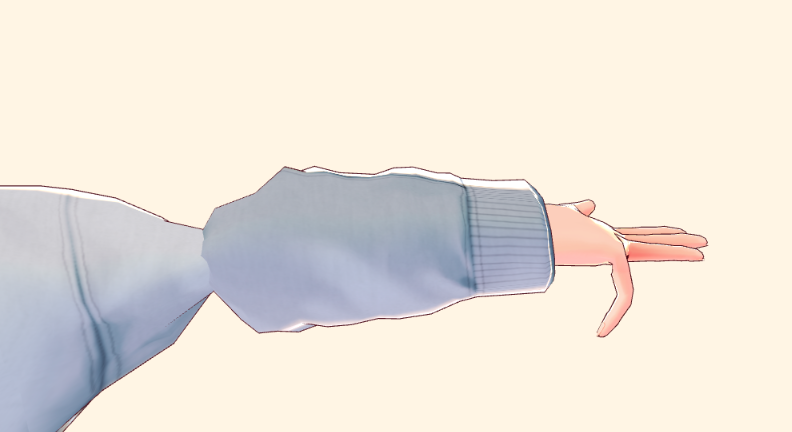
\includegraphics[width=\textwidth]{linear_blend.png}
        \caption{When using linear blend skinning.}
    \end{figure}

    \begin{figure}[H]
        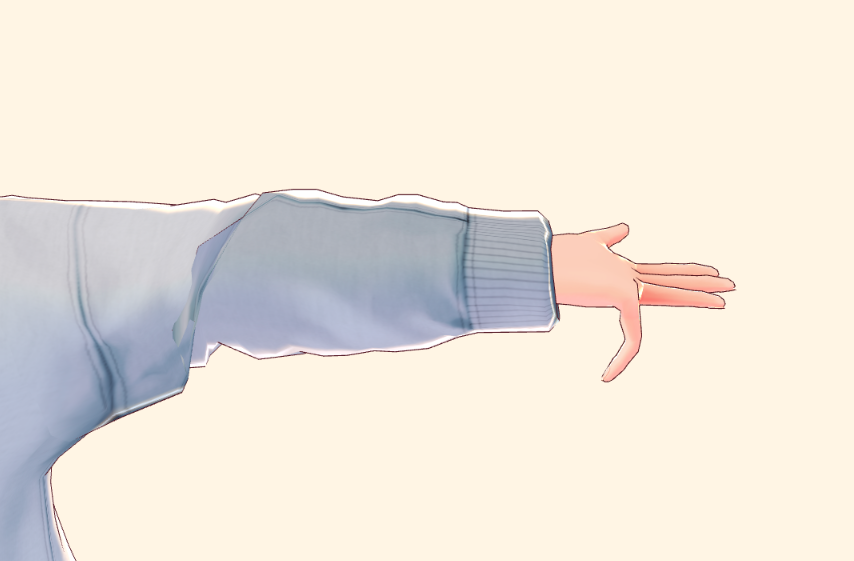
\includegraphics[width=\textwidth]{dual_quat.png}
        \caption{When using dual quaternion skinning.}
    \end{figure}

    One can see a clear difference for the candy wrapper issue with LBS. When seeing carefully, near the joint of the little finger folded in unnatural direction, the model skinned by LBS shows slightly thinner result than one skinned by DQS.

    I'll try to implement other methods as soon as possible!

    \noindent[Disclaimer: The humanoid model is from VRoid Hub. (\url{https://hub.vroid.com/en/characters/1277274004424547671/models/4683457172478674257}) This model can be redistributed according to the conditions of use.]
\end{document}